\documentclass[a4paper,12pt]{article}

\usepackage{Packages}
\usepackage{breqn}
\usepackage{amsmath}
\usepackage{resizegather}
\long\def\/*#1*/{}
\usepackage{listings}

\begin{document}
\begin{titlepage}

\begin{center}

% Upper part of the page. The '~' is needed because \\
% only works if a paragraph has started.

\includegraphics[width=0.6\textwidth]{./Figures/TUe}~\\[2cm]


%\vspace*{10cm}

% Title
\HRule \\[0.4cm]
{ \huge \bfseries 2IMM20 - Foundations of datamining\\[0.3cm] }
\HRule \\[1.5cm]
\textbf{Assignment 2}


% Author and supervisor

\vfill

\begin{table}[h]
\begin{tabular}{ll}
\textbf{Students:} & \\
Joris van der Heijden & (0937329)\\
Bram van der Pol & (0780042)\\

\\
\textbf{Email addresseses:} & \\
j.j.m.v.d.heijden@student.tue.nl \\
a.f.v.d.pol@student.tue.nl \\
\\
\textbf{Supervisors:} &\\
Dr.ir. Joaquin Vanschoren
\\

%\textbf{Supervisors:} & \\
%Dr. M.Holenderski \\
\end{tabular}
\end{table}



% Bottom of the page
\large
{ Eindhoven, \today}

\end{center}


\end{titlepage}
 %included in part 1

\tableofcontents %included in part 1
\newpage

\section{Backpropagation}
\subsection{Math}
\begin{figure}[H]
\hfill
\makebox[\textwidth][c]{{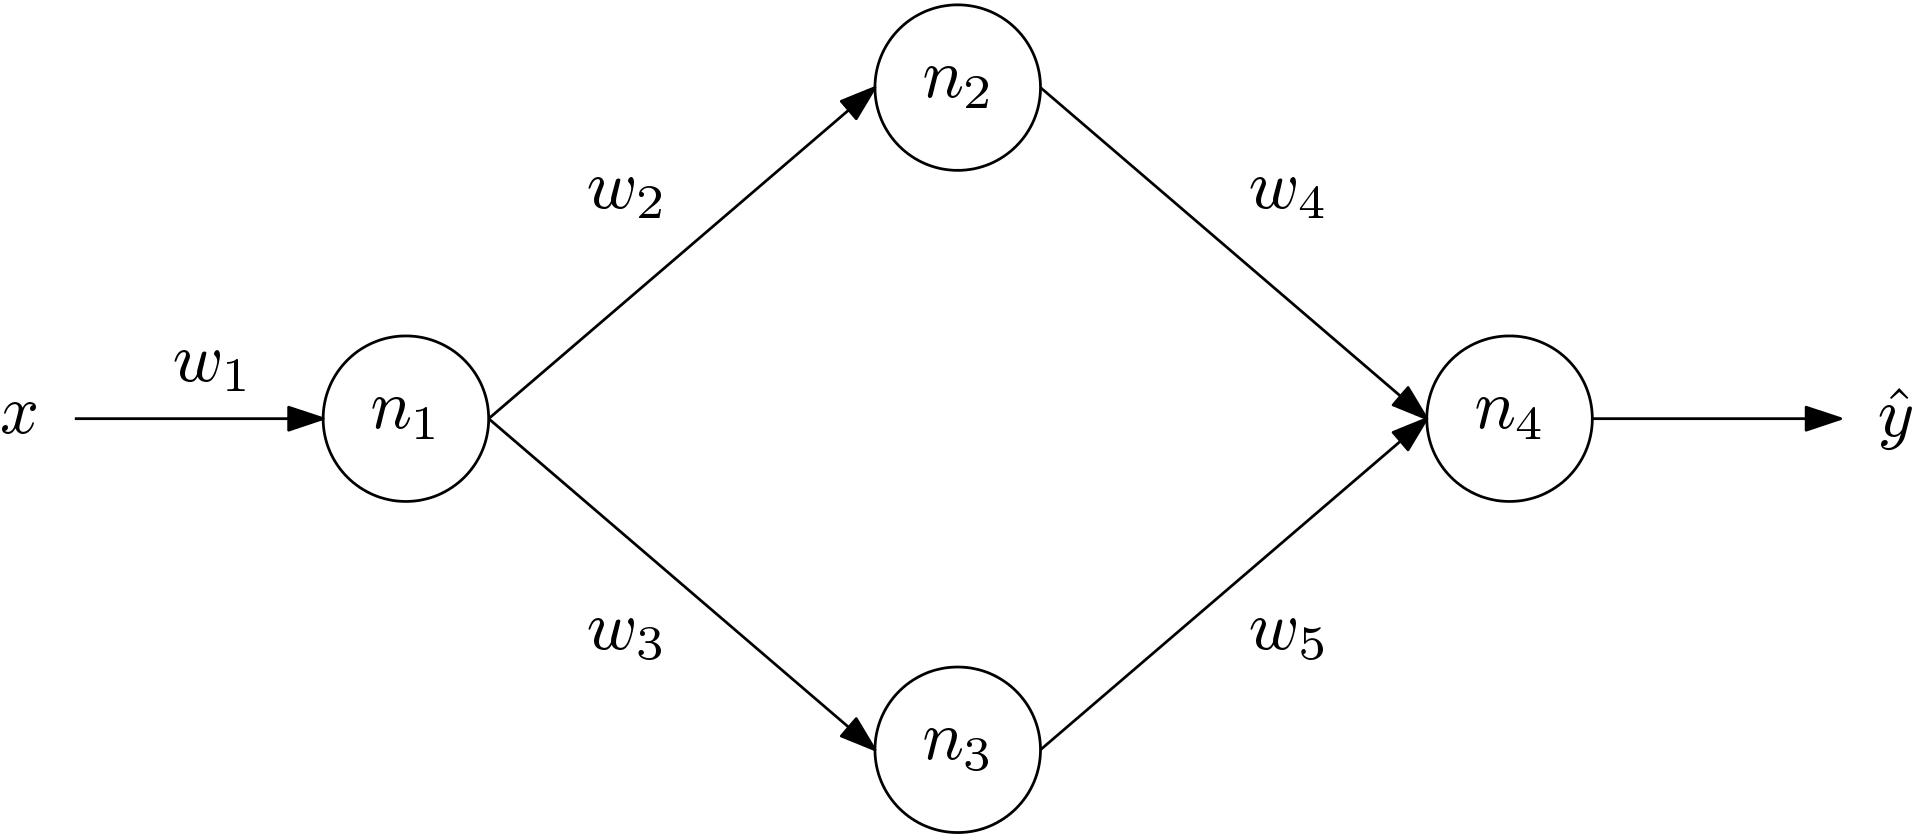
\includegraphics[width=12cm]{./Figures/nn.png}}}
\hfill
\caption{Neural network}
\label{Neural network}
\end{figure}

The activation layers $n$ are given by:

\begin{equation}
\begin{aligned}
n_4 &=\sigma(z_4), \quad z_4 = n_2w_4+n_3w_5   \\
n_3 &= \sigma(z_3),\quad z_3 = n_1w_3 		\\
n_2 &= \sigma(z_2),\quad z_2 = n_1w_2      \\
n_1 &= \sigma(z_1),\quad z_1 = w_1 x
\end{aligned}
\end{equation}

The loss function for 1 sample is given by:
\begin{equation}
\begin{aligned}
L=\frac{1}{2}(n_4-y)^2
\end{aligned}
\end{equation}


The derivatives w.r.t. the weights are given by:

\begin{equation}
\begin{align}
\frac{\partial L}{\partial w_5} &=\frac{\partial C}{\partial n_4}\frac{\partial n_4}{\partial z_4}\frac{\partial z_4}{\partial w_5}=\underbrace{(n_4-y)\sigma'(z_4)}_{\alpha}n_3\\
\frac{\partial L}{\partial w_4} &=\frac{\partial C}{\partial n_4}\frac{\partial n_4}{\partial z_4}\frac{\partial z_4}{\partial w_4}=\alpha n_2\\
\frac{\partial L}{\partial w_3} &= \frac{\partial C}{\partial n_4}\frac{\partial n_4}{\partial z_4}\frac{\partial z_4}{\partial n_3} \frac{\partial n_3}{\partial z_3}\frac{\partial z_3}{\partial w_3} = \alpha w_5\sigma'(z_3)n_1\\
\frac{\partial L}{\partial w_2} &= \frac{\partial C}{\partial n_4}\frac{\partial n_4}{\partial z_4}\frac{\partial z_4}{\partial n_2} \frac{\partial n_2}{\partial z_2}\frac{\partial z_2}{\partial w_2}= \alpha w_4\sigma'(z_2) n_1 \\
\frac{\partial L_{n_2}}{\partial w_1} &= \frac{\partial C}{\partial n_4}\frac{\partial n_4}{\partial z_4}\frac{\partial z_4}{\partial n_2} \frac{\partial n_2}{\partial z_2}\frac{\partial z_2}{\partial n_1}\frac{\partial n_1}{\partial z_1}\frac{\partial z_1}{\partial w_1}= \alpha w_4\sigma'(z_2) w_2 \sigma'(z_1) x\\
\frac{\partial L_{n_3}}{\partial w_1} &= \frac{\partial C}{\partial n_4}\frac{\partial n_4}{\partial z_4}\frac{\partial z_4}{\partial n_2} \frac{\partial n_2}{\partial z_3}\frac{\partial z_3}{\partial n_1}\frac{\partial n_1}{\partial z_1}\frac{\partial z_1}{\partial w_1} =\alpha w_4 \sigma'(z_3) w_3 \sigma'(z_1) x\\
\frac{\partial L}{\partial w_4}&=\frac{\partial L_{n_2}}{\partial w_1}+\frac{\partial L_{n_3}}{\partial w_1}
\end{align}
\end{equation}

The compute graph of the neural network is chosen as a sigmoid: 
\begin{equation}
\begin{aligned}
\sigma(z)=\frac{1}{1+e^{-z}} \\
\sigma'(z)=\frac{e^{-z}}{(exp^{-z} + 1)^2}
\end{aligned}
\end{equation}

The update expressions are given by:
\begin{equation}
\begin{aligned}
w^{new}_i=w_i-\alpha \frac{\partial L}{\partial w_i}, \; i=1,\ldots, 5
\end{aligned}
\end{equation}

First the activation layers are calculated using: ${\bf w}=[2 \; 1 \; 2 \; 4 \; 1]$ and $x=2,\;y=3$.

\begin{equation}
\begin{aligned}
z_1 &= w_1x = 4 \\
z_2 &= n_1w_2 = 0.982  \\
z_3 &= n_1w_3 = 1.964 \\
z_4 &= n_2w_4+n_3w_5=3.787
\end{aligned}
\quad
\begin{aligned}
n_1 &= \sigma(z_1)=0.982  \\
n_2 &= \sigma(z_2)=0.7275 \\
n_3 &=  \sigma(z_3)=0.877 \\
n_4 &=\sigma(z_4)=0.977 
\end{aligned}
\end{equation}
The initial error is: $2.0446$.  
Now by back propagation the new weights are given by:

\begin{equation}
w_{new}^{hand}=\begin{bmatrix} 2.0003 &    1.0034  &   2.0005  &   4.0032  &   1.0038
\end{bmatrix}
\label{eq:handmade}
\end{equation}

The python code:

\begin{lstlisting}
class MyGraph(object):

    def __init__(self, x, y, weigths):
        ''' x: input
            y: expected output
            w: initial weight
            b: initial bias '''
                       
        self.weights = [VariableNode(weight) for weight in weigths]

        self.z1 = MultiplicationNode([ConstantNode(x),self.weights[0]])
        self.n1 = SigmoidNode([self.z1])
        self.z2 = MultiplicationNode([self.n1, self.weights[1]])
        self.n2 = SigmoidNode([self.z2])
        self.z3 = MultiplicationNode([self.n1, self.weights[2]])
        self.n3 = SigmoidNode([self.z3])
        self.z4 = AdditionNode([MultiplicationNode([
                             self.n2,
                             self.weights[3]]),
                             MultiplicationNode([
                             self.n3,
                             self.weights[4]])])
        self.n4 = SigmoidNode([self.z4])
        self.graph = MSENode([self.n4,ConstantNode(y)])

    def forward(self):
        return self.graph.forward()

    def backward(self, d):
        self.graph.backward(d)
    def set_weights(self, new_weights):
        for i in len(new_weights):
            self.weights[i].output = new_weights[i]

    def get_weights(self):
        return [weight.output for weight in self.weights]
\end{lstlisting}
The structure is created using the multiplication and addition nodes. First is started with the $n_1$ node, thereafter the $n_2$ and $n_3$ nodes and finally $n_4$ is constructed using the addition node. This gives the desired shape.

\begin{equation}
w_{new}^{python}=
\begin{bmatrix} 2.000 &   1.003 & 2.000    4.003 & 1.004
\end{bmatrix}
\label{eq:python}
\end{equation}

As can been seen in \ref{eq:handmade} and \ref{eq:python} is that the handmade calculations are more accurate but the numbers calculated by the python code are equal to the handmade calculations. 


\section{Assignment 2}


%\begin{figure}
%    \centering
%    \begin{subfigure}[b]{0.3\textwidth}
%        \includegraphics[width=\textwidth]{\figures\•}
%        \caption{•}
%        \label{fig:•}
%    \end{subfigure}
%
%    \begin{subfigure}[b]{0.3\textwidth}
%        \includegraphics[width=\textwidth]{\figures\•}
%        \caption{•}
%        \label{fig:•}
%    \end{subfigure}
%\end{figure}

\section{Assignment 3}
Intuitively, the keras model consists of two parts. In the first part, the input images are converted into numbers, and in the second part these numbers are summed. A network design for these two parts separately was given, so the idea was to link them together.\\

The first part of the network consist of a Dense(128) relu layer for recognising a single image, just like in the example. This layer was followed by a Dense(10) sigmoid that is intended to recognize a number between 0 and 9. This was duplicated 10 times for each of the 10 images. This network should be able to learn to recognise a digit from an image.

To link the first part to the second part, a flatten layer was inserted such that the output of the 10 image recognition layers could be the input for the RNN. The second part is basically the same RNN(128) network used to sum two numbers as given in the example, but with an extra hidden layer and with a different output length. This part should be able to learn how to sum the images. To do so, a TimeDistributed layer with 10 neurons was added in order to generate the sum. The output layer consists of Dense(90) sigmoid layer that determines the final output class, that is the sum of the 10 images. Since each image has a value of [0-9], summing 10 images yields sums in the [0-90] range.
After 30 epochs this resulted in a validation accuracy of 0.45.\\

To try and improve efficiency, a new Dense(784) layer was placed in front of the previous Dense(128) layer. The idea was that a network with a neuron for each pixel of an input image might improve the accuracy. Furthermore, a second layer was added to the RNN. After these modifications a validation accuracy of 0.65 resulted after 30 epochs.\\

The first part would have been more efficient if a single network was trained to recognise one image, which could then be used to do the recognition for each of the 10 images, but we were unable to get that to work properly. This also meant the training set had to be larger such that each of the 10 individual image recognition layers could learn to recognise number properly. For 10 images this architecture works fine, but if the network were to be adapted to handle larger sums, this approach will reach its limits. However, for 10 images the training of the network is still not an issue on a normal desktop machine.


\end{document}
